\documentclass{beamer}

\usepackage[utf8]{inputenc}
\usepackage[english]{babel}

\usepackage{graphicx}
\usepackage{amsmath}
\usepackage{amssymb}
\usepackage{amsthm}
\usepackage{array}

\usepackage{alltt}

\addtocounter{footnote}{1}
\setcounter{tocdepth}{5}
\setcounter{secnumdepth}{5}
\renewcommand{\floatpagefraction}{0.75}

%Information to be included in the title page:
\title{Recap: Concurrency Control}
\author{Alexander Christensen}
\institute{Department of Computer Science \\ University of Copenhagen}
\date{2019}

%% Reference an equation, a figure, or a section

%% \secref{label} - make a reference to a section
\newcommand{\secref}[1]{Section~\ref{#1}}

%% \eqref{reference} - make a reference to an equation
%%\newcommand{\eqref}[1]{(\ref{#1})}

%% \figref{reference} - make a reference to an figure
\newcommand{\figref}[1]{Figure~\ref{#1}}

\newcommand{\basetop}[1]{\vtop{\vskip-1ex\hbox{#1}}}
\newcommand{\source}[1]{\let\thefootnote\relax\footnotetext{\scriptsize\textcolor{kugray1}{Source: #1}}}

%\bibliographystyle{longalpha}
%\bibliography{refs}

%% -*- Mode: latex -*-

%% Macros defined during a long time and used much
% plus - a plus sign
\newcommand{\plus}{+}

% minus - a minus having the same width as a plus
\newlength{\minuswidth}
\settowidth{\minuswidth}{+}
\newlength{\minusheight}
\settoheight{\minusheight}{+}
\newcommand{\minus}{\rule[0.5\minusheight]{\minuswidth}{0.5pt}}

% The basis vector standard
%\renewcommand{\vec}[1]{\boldsymbol{#1}}
\newcommand{\grad}{\operatorname{\nabla}}
\newcommand{\curl}{\operatorname{\text{curl}}}
\newcommand{\divergence}{\operatorname{\text{div}}}
\newcommand{\vecop}{\operatorname{\text{vec}}}
\newcommand{\diag}{\operatorname{\text{diag}}}
\renewcommand{\Re}{\mathbb{R}}
\newcommand{\Co}{\mathbb{C}}
\newcommand{\In}{\mathbb{Z}}
\newcommand{\sign}{\operatorname{sgn}}
%\newcommand{\trace}{\operatorname{Tr}}
\newcommand{\arctantwo}{\ensuremath{\arctan\!2}}
%\newcommand{\mat}[1]{\ensuremath{\boldsymbol{#1} }}
\newcommand{\I}{\mat{1}}
\newcommand{\crossmat}[1]{\ensuremath{\boldsymbol{#1}^{\times} }}
\newcommand{\jacobian}[1]{\ensuremath{\boldsymbol{\mathit{#1}} }}
\newcommand{\set}[1]{\ensuremath{ \boldsymbol{#1} }}
\newcommand{\func}[1]{{\bf{#1}}}
\newcommand{\enorm}[1]{\ensuremath{\left\| #1 \right\|_{_2}}}
%\newcommand{\norm}[1]{\ensuremath{\left\| #1 \right\|}}
\newcommand{\bdet}[1]{\ensuremath{\left| #1 \right|}}
\newcommand{\abs}[1]{\ensuremath{\left| #1 \right|}}
\newcommand{\rtm}{$^{\textrm{®}}$}


\newcommand{\kenny}[1]{ #1 }
\newcommand{\henrik}[1]{ #1 }


%% \maya - the maya signature
\newcommand{\maya}{$ \texttt{Maya}^{\text{\texttrademark}} $}

%% \fat{symbol} - make this symbol fat
\newcommand{\fat}[1]{\mathit{\mathbf{#1}}}
%% \newcommand{\fat}[1]{\hbox{\boldmath $ #1 $}}

%% \vec{symbol} - Vector
%% \renewcommand{\vec}[1]{\mathbf{#1}}
\renewcommand{\vec}[1]{\fat{#1}}

%% \mat{symbol} - Matrix
%%\newcommand{\mat}[1]{\ensuremath{\boldsymbol{#1} }}
\newcommand{\mat}[1]{\fat{#1}}

%% \ezero,...,\ethree - the spin matrices
\newcommand{\ezero}{\begin{bmatrix} 1 & 0 \\  0 &  1 \end{bmatrix}}
\newcommand{\eone}{\begin{bmatrix} i & 0 \\  0 & -i \end{bmatrix}}
\newcommand{\etwo}{\begin{bmatrix} 0 & 1 \\ -1 &  0 \end{bmatrix}}
\newcommand{\ethree}{\begin{bmatrix} 0 & i \\  i &  0 \end{bmatrix}}

%% \quat{symbol} - Quaternion
%% \newcommand{\quat}[1]{\mathbf{#1}}
\newcommand{\quat}[1]{\fat{#1}}

%% \real{quaternion} - the real (scalar) part of a quaternion
\newcommand{\real}{\operatorname{real}}

%% \pure{quaternion} - the pure (vector) part of a quaternion
\newcommand{\pure}{\operatorname{pure}}

%% \sgn{symbol} - the sign of a symbol
\newcommand{\sgn}{\operatorname{sgn}}

%% \norm{symbol} - Norm of a vector/quaternion
\newcommand{\norm}[1]{\parallel {#1} \parallel}

%% \trace{matrix}
\newcommand{\trace}[1]{\mathrm{trace}(#1)}

% This is for code-snippets in the text.
\usepackage{fancyvrb}   %% Try to comment this out if problems with pdflatex
\newcommand{\code}[1]%
%{ \VerbatimInput[frame=none,fontsize=\footnotesize,numbers=none,label=\texttt{#1}]{#1}  }
{ \VerbatimInput[frame=single,fontsize=\footnotesize,numbers=left,label=\texttt{#1}]{#1}  }


%\newcommand{\todo}[1]{ {\Bf Todo:} #1}
\newcommand{\todo}[1]{ }

%\newcommand{\longversion}[1]{ #1 }
\newcommand{\longversion}[1]{ }


\mode<presentation>
{
  \usetheme{Diku}
  \beamertemplatenavigationsymbolsempty
  \setbeamercovered{invisible}
%  \setbeamercovered{transparent=15}
}

%% Kennys pseudocode environment

\newenvironment{pseudocode}{
  \begin{center}
    \begin{minipage}[t]{0.8\columnwidth}
      \footnotesize
      \rule{\columnwidth}{1pt}
    }{
      \rule{\columnwidth}{1pt}
    \end{minipage}
  \end{center}
}

{
\AtBeginSection[wef]
{
\begin{frame}
\frametitle{Table of Contents}
\tableofcontents[currentsection]{1}
\end{frame}
}
}


\begin{document}

% Set background to front page
\usebackgroundtemplate{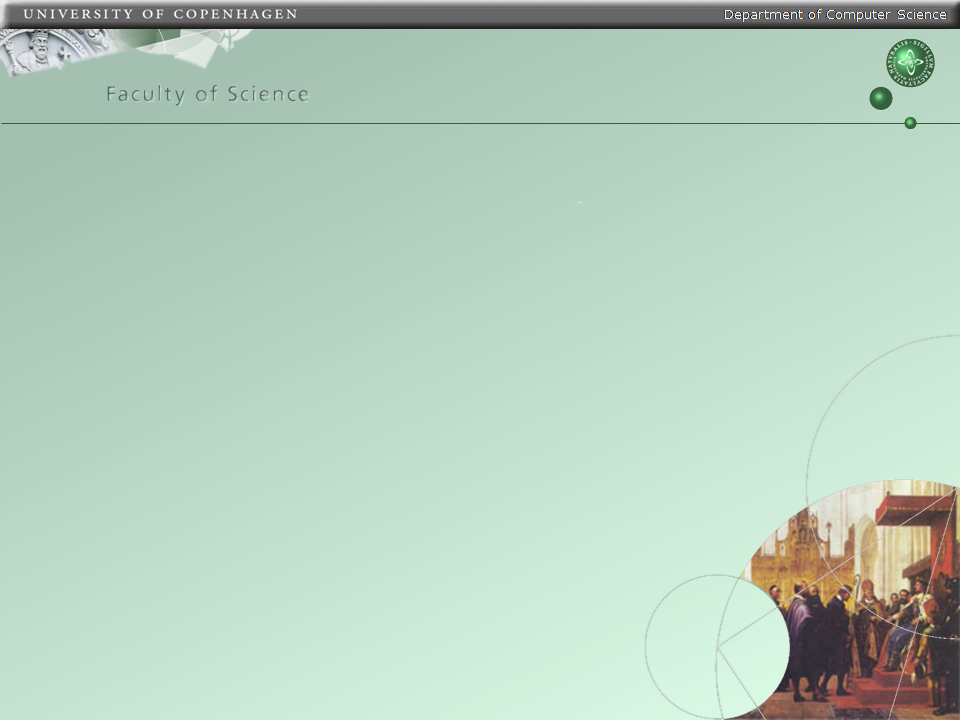
\includegraphics[width=\paperwidth,height=\paperheight]{front}}
{
\begin{frame}[plain]
  \titlepage
\end{frame}
}

% Set background to rest of pages
\usebackgroundtemplate{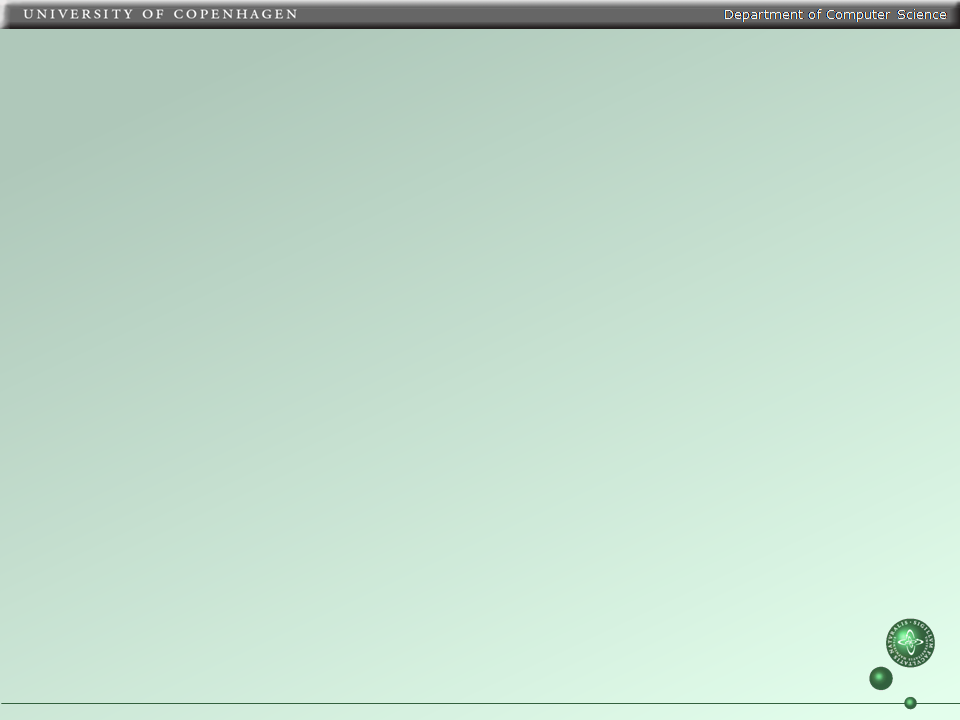
\includegraphics[width=\paperwidth,height=\paperheight]{background}}

%
%
%
\begin{frame}
\frametitle{Overview}
\tableofcontents
\end{frame}



%
%
%
\begin{frame}
\frametitle{What is concurrency?}
\section{What is concurrency?}

"Logical control flows are \textit{concurrent} if they overlap in time."
\footnote{\ (BOH, cp. 12)\vspace{2mm}}

\begin{figure}
\includegraphics[width=0.8\textwidth]{images/concurrent-processes.png}
\end{figure}
\end{frame}



%
%
%
\begin{frame}
\frametitle{How can we achieve concurrency?}
\section{How can we achieve concurrency?}
We have 3 different set of tools available to use for writing
concurrent programs:\\
\vspace{3mm}
\textbf{Processes}
\begin{itemize}
\item A running program can clone itself into one or more child processes
\item Completely separated memory areas
\end{itemize}
\vspace{2mm}

\textbf{I/O Multiplexing}
\begin{itemize}
\item Resembles event-driven programming
\item I/O operations do not block
\end{itemize}
\vspace{2mm}

\textbf{Threading}
\begin{itemize}
\item Multiple parallel control flows exist within the same process
\item Often the most practical solution
\end{itemize}
\end{frame}



%
%
%
\begin{frame}
\frametitle{Processes}
\subsection{Processes}
How do we use them?

\begin{figure}
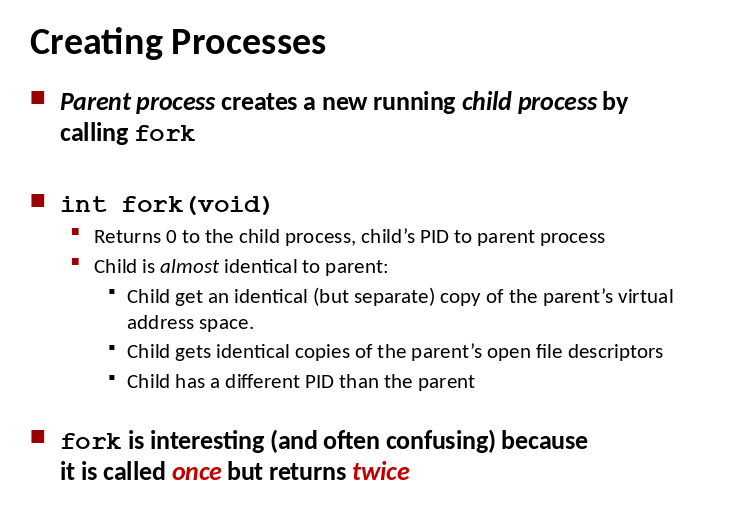
\includegraphics[width=0.8\textwidth]{images/creating-processes.png}
\end{figure}

\end{frame}



%
%
%
\begin{frame}
\frametitle{Processes}
Exam question from re-exam 19/20:

\vspace{-3mm}
\begin{figure}
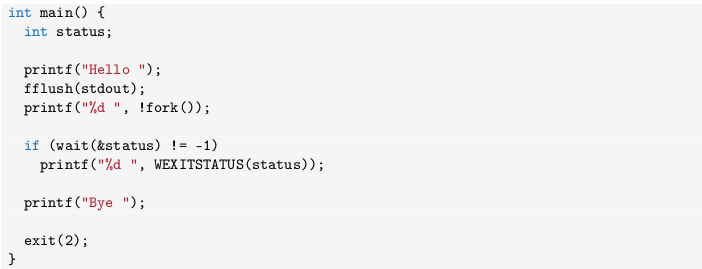
\includegraphics[width=1.0\textwidth]{images/exam_question_1_fork.png}
\end{figure}
\vspace{-3mm}
Which of the following are \textit{possible} valid outputs of the program?
\vspace{2mm}

\begin{columns}
\begin{column}{0.5\textwidth}
\footnotesize
\ \ \ \ \textbf{a)} \texttt{Hello 0 1 Bye 2 Bye}\\
\ \ \ \ \textbf{b)} \texttt{Hello Bye 1 0 2 Bye}\\
\ \ \ \ \textbf{c)} \texttt{Hello 1 0 Bye 2 Bye}
\end{column}
\begin{column}{0.5\textwidth}  %%<--- here
\footnotesize
\textbf{d)} \texttt{Hello 1 Bye 0 2 Bye}\\
\textbf{e)} \texttt{Hello 0 Bye 1 2 Bye}\\
\textbf{f)} \texttt{Hello 0 1 Bye Bye 2}
\end{column}
\end{columns}

\end{frame}


%% %
%% %
%% %
%% \section{Texture Mapping}
%% \begin{frame}
%% Given a triangle with texture coordinates $(u1,v1)$, $(u2,v2)$, and $(u3,v3)$,
%% we employ a mapping, such that each vertex gets its own texture coordinate.
%% \frametitle{Texture Mapping}
%% \begin{figure}
%% \includegraphics[width=0.9\textwidth]{images/textureMapping.png}
%% \end{figure}
%% \end{frame}


%
%
%
\begin{frame}
\frametitle{Texture mapping}
OpenGL performs texture mapping automatically, based on the chosen filtering
function, and the \textit{interpolation quilifiers} that we specify in our
fragment shader:

\begin{alltt}\footnotesize
in vec2 texCoord; // default : perspective-correct interpolation\\

smooth in vec2 texCoord; // the same\\

noperspective in vec2 texCoord; // smooth, but not perspective-correct\\

flat in vec2 texCoord; // no interpolation
\end{alltt}
\end{frame}


%
%
%
\begin{frame}
\frametitle{Reading an image from disk}
Assume a 2D texture with four color channels (RGBA) stored as a file
\texttt{"ourImage.png"}:

\begin{alltt}\footnotesize
int width, height;\\
GLubyte* ourTextureData = someFunctionToReadFromDisk("ourImage.png",\\
\ensuremath{\qquad}\&width, \&height);\\

GLuint ourTexture;\\
glGenTextures(1, \&ourTexture);\\
glBindTexture(GL\_TEXTURE\_2D, ourTexture);\\
glTexImage2D(GL\_TEXTURE\_2D, 0, GL\_RGBA, width, height, 0, GL\_RGBA,\\
\ensuremath{\qquad}GL\_UNSIGNED\_BYTE, ourTextureData);\\

// remember to cleanup once the image is buffered to the GPU\\
delete ourTextureData;\\
\end{alltt}
\end{frame}


%
%
%
\begin{frame}
\frametitle{What is a Texture - Binding the texture}
To use our texture, it must be bound within the context of an activated
shader program:

\begin{alltt}\footnotesize
// activate our shader as the current program in\\
// OpenGL's state machine\\
GLuint ourShader = SomeFunctionToCreateAShader();\\
glUseProgram(ourShader);\\
\end{alltt}

Now we need to bind the texture to texture unit \#0:
\begin{alltt}\footnotesize
glActiveTexture(GL\_TEXTURE0);\\
glBindTexture(GL\_TEXTURE\_2D, ourTexture);
\end{alltt}

Maximum number of texture units (simultaneously bound textures) can be queried:
\begin{alltt}\footnotesize
int maxTextureUnits = 0;\\
glGetIntegerv(GL\_MAX\_TEXTURE\_UNITS, \&maxTextureUnits);
\end{alltt}
\end{frame}


%
%
%
\begin{frame}
\frametitle{Using the texture in a rendering call}
When the texture is bound we tell the shader where to find it:
\begin{alltt}\footnotesize
GLint location = glGetUniformLocation(ourShader,\\
\ensuremath{\qquad}"nameInFragmentShader");\\
glUniform1i(location, 0); // 0 corresponds to the chosen texture unit
\end{alltt}

Now the texture is bound within the shader, and we have buffered its
position on the GPU as well. Now we can use our rendering commands to render
the texture onto our surface.
\end{frame}


\begin{frame}
\frametitle{Texture Mapping - Vertex Shader}
The texture coordinate should be buffered together with the vertex position,
as a per-vertex attribute:
\begin{alltt}\footnotesize
\#version 330 core\\

layout (location = 0) in vec2 vertexPos;\\
layout (location = 1) in vec2 texCoord;\\

out vec2 interpolatedTexCoord;\\

void main()\\
\{\\
\ensuremath{\qquad}gl\_Position = vec4(vertexPos, 0.0f, 1.0f);\\
\ensuremath{\qquad}interpolatedTexcoord = texCoord; // will be interpolated by OpenGL\\
\}
\end{alltt}
\end{frame}


%
%
%
%% \begin{frame}
%% Any input/output variable between vertex- and fragment shader is
%% automatically interpolated by OpenGL.
%% \frametitle{Texture Mapping - Fragment Shader}
%% \begin{alltt}\footnotesize
%% \#version 330 core\\

%% uniform sampler2D textureSampler;\\
%% in vec2 interpolatedTexCoord;\\
%% out vec4 color;\\

%% void main()\\
%% \{\\
%% \ensuremath{\qquad}color = texture(textureSampler, interpolatedTexcoord);\\
%% \}
%% \end{alltt}
%% \end{frame}


%% \section{Examples}
%% %
%% %
%% %
%% \begin{frame}
%% \frametitle{Example with 1 texture}
%% Render a two triangles with 1 texture mapped onto them.
%% \end{frame}


%
%
%
\begin{frame}
\frametitle{Example with 2 textures}
Render two triangles, but this time buffer two textures and perform various
smooth transitioning effects between them based on the cursor position
on the screen.
\end{frame}


\section{What can go wrong in concurrent programs}
%
%
%
%% \begin{frame}
%% \frametitle{The bigger perspective - Framebuffers}
%% Textures are images loaded to GPU memory.

%% We are not restricted only to reading from textures,
%% we an also write to them.

%% \begin{figure}
%% \includegraphics[width=0.8\textwidth]{lecture-slides/concurrent-processes.png}
%% \end{figure}
%% If we have $N-1$ textures, and let $N$ represent the application window,
%% then for $1 \leq i \leq N - 1$ we can use the image data in texture $i$
%% to run a shader which writes to texture $i+1$. The final image in
%% texture $N$ is rendered to the screen.
%% \end{frame}


%
%
%
\begin{frame}
\frametitle{Framebuffer Example: Conway's Game of Life}
\textbf{Idea:}\\
Use a framebuffer with 2 textures attached, use one for reading,
the other for writing.\\\vspace{4mm}

\textbf{Algorithm:}\\
Bind the framebuffer. Make a drawing call to read from \texttt{read}
texture and write to \texttt{write} texture. Unbind the framebuffer.
Make a drawing call again with \texttt{write} texture as uniform.
Swap \texttt{read} and \texttt{write}.
\end{frame}


%
%
%
\begin{frame}
\frametitle{The bigger perspective - Inspiration}
Many common 3D rendering techniques use textures:

\begin{itemize}
\item normal mapping
\item bump mapping
\item parallax mapping
\item static illumination
\end{itemize}

\vspace{4mm}
Many common 3D rendering techniques rely on framebuffers:

\begin{itemize}
\item deferred rendering
\item shadow mapping
\item screen-space ambient occlusion (SSAO)
\item fast approximate anti-aliasing (FXAA)
\end{itemize}

\end{frame}


%
%
%
\begin{frame}
\frametitle{Summary}
We have seen the texture coordinate system.

\vspace{5mm}
We have looked at techniques for filtering, clamping, and wrapping
of textures.

\vspace{5mm}
We have seen how textures can be used to enhance visual effects.

\vspace{5mm}
Some code examples have shown how textures can be used in OpenGL 3.3.
\end{frame}


%
%
%
%% \begin{frame}
%% \frametitle{References}
%% \nocite{*}
%% \bibliography{refs}{}
%% \bibliographystyle{alpha}
%% \end{frame}



\end{document}
